\chapter{Анализ технологического процесса 3D-печати и причин возникновения дефектов}

\section{Технология послойного наплавления: принципы, ограничения и критичные параметры процесса}

В данной работе рассматривается технология печати методом послойного наплавления, для которой разрабатывается контур мониторинга и раннего обнаружения отклонений. Метод послойного наплавления (Fused Deposition Modeling, FDM)~\textemdash{} аддитивный метод, при котором полимерная нить подается в нагревательный блок, расплавляется и через сопло наносится слоями, формируя геометрию изделия~\cite{лысыч2014области}.

Схема устройства FDM-принтера приведена на рисунке~\ref{fig:FDM}.

\begin{figure}[h!]
\centering
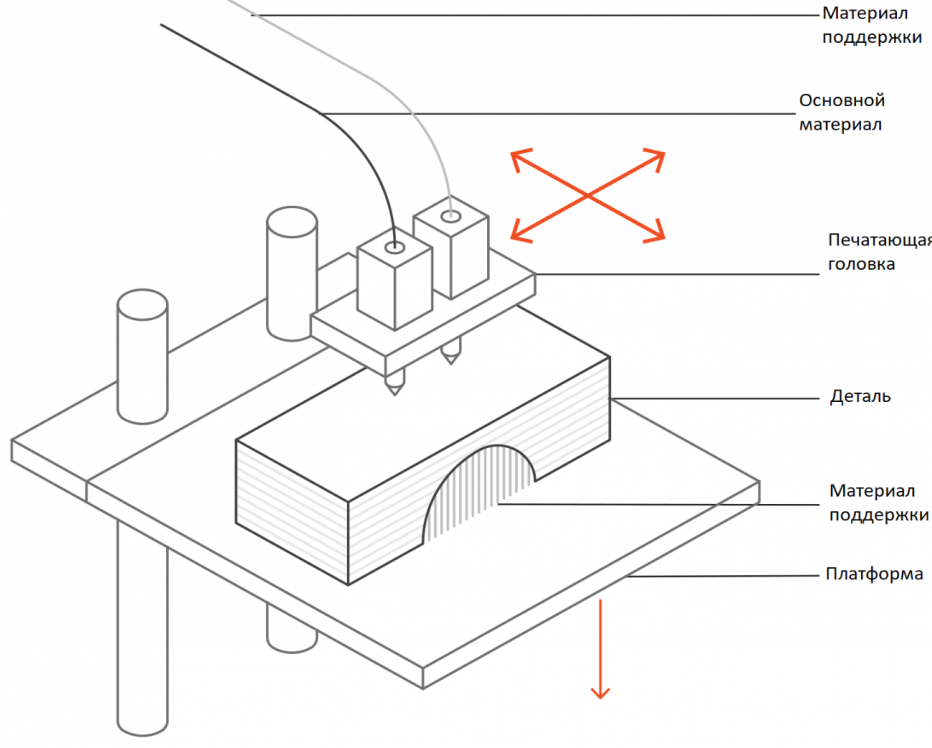
\includegraphics[width=0.75\hsize]{fig/FDM.png}
\caption{Схема устройства FDM-принтера}
\label{fig:FDM}
\end{figure}

Технологический цикл включает подготовку модели, формирование управляющей траектории и построение изделия слоями. Качество печати зависит от материала, состояния оборудования, внешних условий и цифровой подготовки задания. Возникшее отклонение может влиять на последующие слои и усиливаться по мере построения изделия.

С практической точки зрения дефекты FDM-печати целесообразно рассматривать как следствие нарушения устойчивости процесса. Если в одном из звеньев технологической цепочки возникает отклонение, оно влияет и на последующие слои и может усиливаться по мере печати изделия.
Филамент~\textemdash{} полимерный расходный материал в виде непрерывной нити заданного диаметра, подаваемой в экструдер. Его свойства влияют на стабильность экструзии, межслойную адгезию и геометрию изделия.

Нестабильный диаметр нити вызывает колебания объема расплавляемого материала и нарушает равномерность слоя. Контакт сопла с неровностями детали может привести к смещению слоев или дефекту типа «спагетти». Влага при нагреве образует пузырьки в расплаве, ухудшая межслойную адгезию и способствуя растрескиванию. Пыль и мусор на нити могут засорять экструдер и сопло, вызывая заедания, пропуски шагов и неравномерную подачу материала вплоть до срыва печати.

Перегибы нити, повышенное трение и нестабильная намотка на катушке могут нарушать подачу материала или вызывать заедание механизма. Эти нарушения также могут привести к дефекту типа «спагетти» или смещению слоев.

Со стороны оборудования причинами отклонений служат люфты, износ и загрязнение механических узлов, нестабильность перемещений и недостаточная повторяемость позиционирования. Погрешности первых слоев могут накапливаться и проявляться позднее как смещение слоев или потеря точности. Заедания, перегрузки и нестабильная работа приводов особенно критичны для длительных заданий и могут привести к отказу кинематики.

Колебания температуры, сквозняки и контакты с посторонними предметами могут нарушать тепловой режим и создавать механические помехи. Неравномерное охлаждение из-за сквозняка может ухудшать адгезию и способствовать растрескиванию. Случайное прикосновение к печатающей голове может вызвать смещение слоев или повреждение оборудования.

\section{Классы дефектов печати и факторы их возникновения в реальных условиях эксплуатации}

Для визуального мониторинга важны критичные для процесса дефекты, различимые по изображениям рабочей зоны.

С инженерной точки зрения дефекты различаются по последствиям: ухудшение геометрии и внешнего вида изделия, снижение прочности, срыв задания и риск повреждения принтера. Задержка обнаружения также увеличивает потери материала и машинного времени.

Для сопоставления рассматриваются растрескивание, отлипание модели от стола, смещение слоев и дефект типа «спагетти».

Растрескивание отражает нарушение целостности изделия и связано с потерей межслойной адгезии. На практике этот дефект проявляется при неблагоприятном тепловом режиме и неравномерном охлаждении. Даже локальные трещины ухудшают эксплуатационные свойства детали и могут сделать ее непригодной для применения.

Отлипание модели от стола является критическим дефектом начальной стадии, поскольку нарушает базовую геометрию дальнейшего построения. Причинами обычно выступают неверный зазор сопла и пластины на первом слое и загрязнение стола. При потере контакта первого слоя с поверхностью изделие начинает смещаться, что приводит к срыву печати.

Смещение слоев возникает, когда траектория укладки материала сдвигается относительно ранее сформированной части изделия. Визуально это проявляется в виде ступенчатого смещения и несоосности стенок. Причинами обычно становятся пропуски шагов двигателями, перегрузка кинематики, недостаточное натяжение ремней, заедание механики или столкновение с деформированным изделием.

Отлипание или смещение модели может нарушить контакт экструдируемого материала с уже напечатанной частью изделия. При продолжении подачи пластик накапливается в виде хаотичных нитей, образуя дефект типа «спагетти». Задание фактически выполняется вхолостую, а восстановление рабочего состояния принтера затрудняется.

Характерное проявление дефекта типа «спагетти» приведено на рисунке~\ref{fig:spaghetti-yellow}.

\begin{figure}[h!]
  \centering
  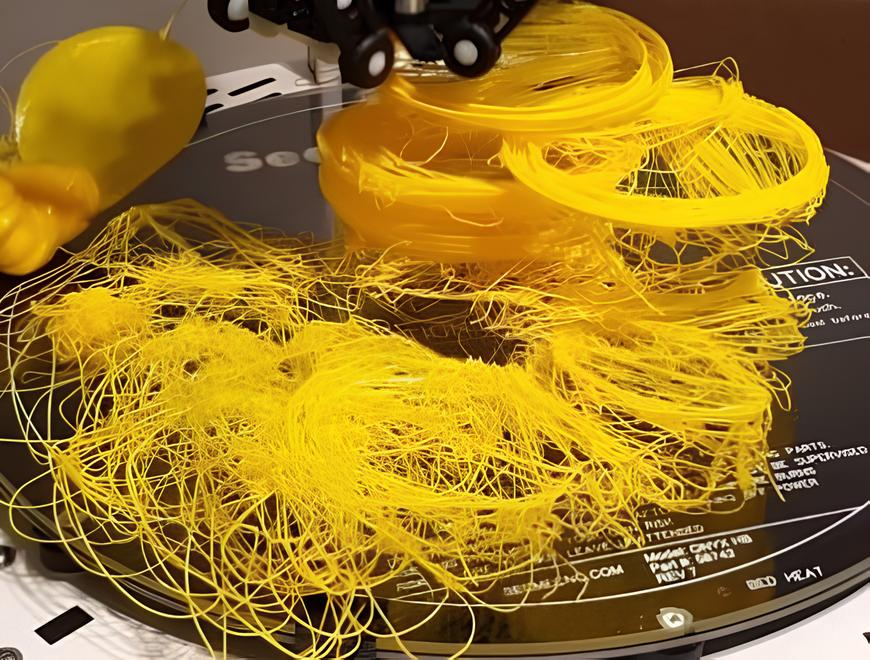
\includegraphics[width=0.56\hsize]{fig/spag.jpeg}
  \caption{Дефект типа «спагетти» при частичном разрушении печатаемой модели}
  \label{fig:spaghetti-yellow}
\end{figure}

На рисунке нити выходят за пределы модели и уже не образуют заданную геометрию. Отдельные тонкие нити при перемещении сопла сами по себе не доказывают срыв печати. Признаками дефекта служат накопление материала вне модели и сохранение этого проявления на последовательных кадрах.

Таким образом, на первом этапе модель обучается обнаруживать только дефект типа «спагетти». Он требует быстрой реакции из-за потерь материала и машинного времени, а хаотичные нити хорошо различимы на изображениях.

\iffalse
\begin{table}[ht]
\caption{Сводная характеристика приоритетных дефектов для раннего обнаружения}
\label{table:defects_priority}
\scriptsize
\renewcommand{\arraystretch}{1.05}
\setlength{\tabcolsep}{3pt}
\centering
\begin{tabular}{|>{\raggedright\arraybackslash}m{70pt}|>{\raggedright\arraybackslash}m{86pt}|>{\raggedright\arraybackslash}m{88pt}|>{\raggedright\arraybackslash}m{58pt}|>{\raggedright\arraybackslash}m{86pt}|}
\hline
Дефект & Ранние визуальные признаки & Влияние на процесс & Приоритет реагирования & Базовое действие системы \tabularnewline
\hline
Растрескивание & Трещины, расхождение слоев, нарушение поверхности & Потеря прочности, риск перехода в дефект «спагетти» & Высокий & Фиксация события, уведомление, контроль динамики \tabularnewline
\hline
Отлипание модели от стола & Смещение модели, потеря контакта первого слоя со столом & Деформация геометрии, риск перехода в дефект «спагетти» & Критический & Немедленная пауза и остановка при подтверждении отклонения \tabularnewline
\hline
Дефект типа «спагетти» & Хаотичные нити пластика вне контура модели & Бесполезный расход материала, потеря машинного времени & Критический & Остановка задания, уведомление, подготовка к перезапуску \tabularnewline
\hline
Смещение слоев & Ступенчатый сдвиг контуров, несоосность слоев & Искажение геометрии, риск непригодности детали и перехода в дефект «спагетти» & Высокий & Фиксация события, уведомление, пауза при подтверждении отклонения \tabularnewline
\hline
\end{tabular}
\end{table}
\fi

Для оценки результатов выполнения заданий в реальных условиях собрана эксплуатационная статистика фермы 3D-принтеров компании Stereotech. Сбор выполнен~15~мая~2026~года. Данные получены с десяти доступных устройств. Сводка охватывает всю сохраненную историю каждого принтера без ограничения по периоду. Для анализа использованы статусы заданий, накопленное время печати и расход филамента.

Сводные показатели эксплуатации и количество заданий по статусам представлены в таблице~\ref{table:stereotech-print-statistics}.

\begin{table}[!ht]
\caption{Сводные показатели эксплуатации фермы 3D-принтеров компании Stereotech}
\label{table:stereotech-print-statistics}
\centering
\small
\renewcommand{\arraystretch}{1.05}
\begin{tabular}{|l|r|}
\hline
Показатель & Значение \tabularnewline
\hline
Количество принтеров & 10 \tabularnewline
\hline
Общее время печати & 765~д 7~ч 38~мин 21~с \tabularnewline
\hline
Максимальное время одного задания & 4~д 17~ч 17~мин 21~с \tabularnewline
\hline
Среднее время одного задания & 3~ч 56~мин 8~с \tabularnewline
\hline
Расход филамента & 51\,760,1~м \tabularnewline
\hline
Задания по общему счетчику & 4\,667 \tabularnewline
\hline
Задания с известным статусом & 4\,640 \tabularnewline
\hline
Завершено & 3\,063 \tabularnewline
\hline
Отменено & 1\,237 \tabularnewline
\hline
Аварийная остановка & 244 \tabularnewline
\hline
Ошибка & 72 \tabularnewline
\hline
Ошибка системы & 12 \tabularnewline
\hline
Неудачно & 12 \tabularnewline
\hline
\end{tabular}
\end{table}

Общее время печати и расход филамента суммированы по доступным устройствам. Средняя продолжительность получена делением суммарного времени на число заданий по общему счетчику, максимальная выбрана среди зарегистрированных значений принтеров.

Распределение заданий по статусам приведено на рисунке~\ref{fig:stereotech-print-statuses}. Завершенные задания составляют~66,0~\%, отмененные~\textemdash{} 26,7~\% от числа заданий с известным статусом. Подписи этих долей на диаграмме округлены до целых процентов.

\begin{figure}[!ht]
  \centering
  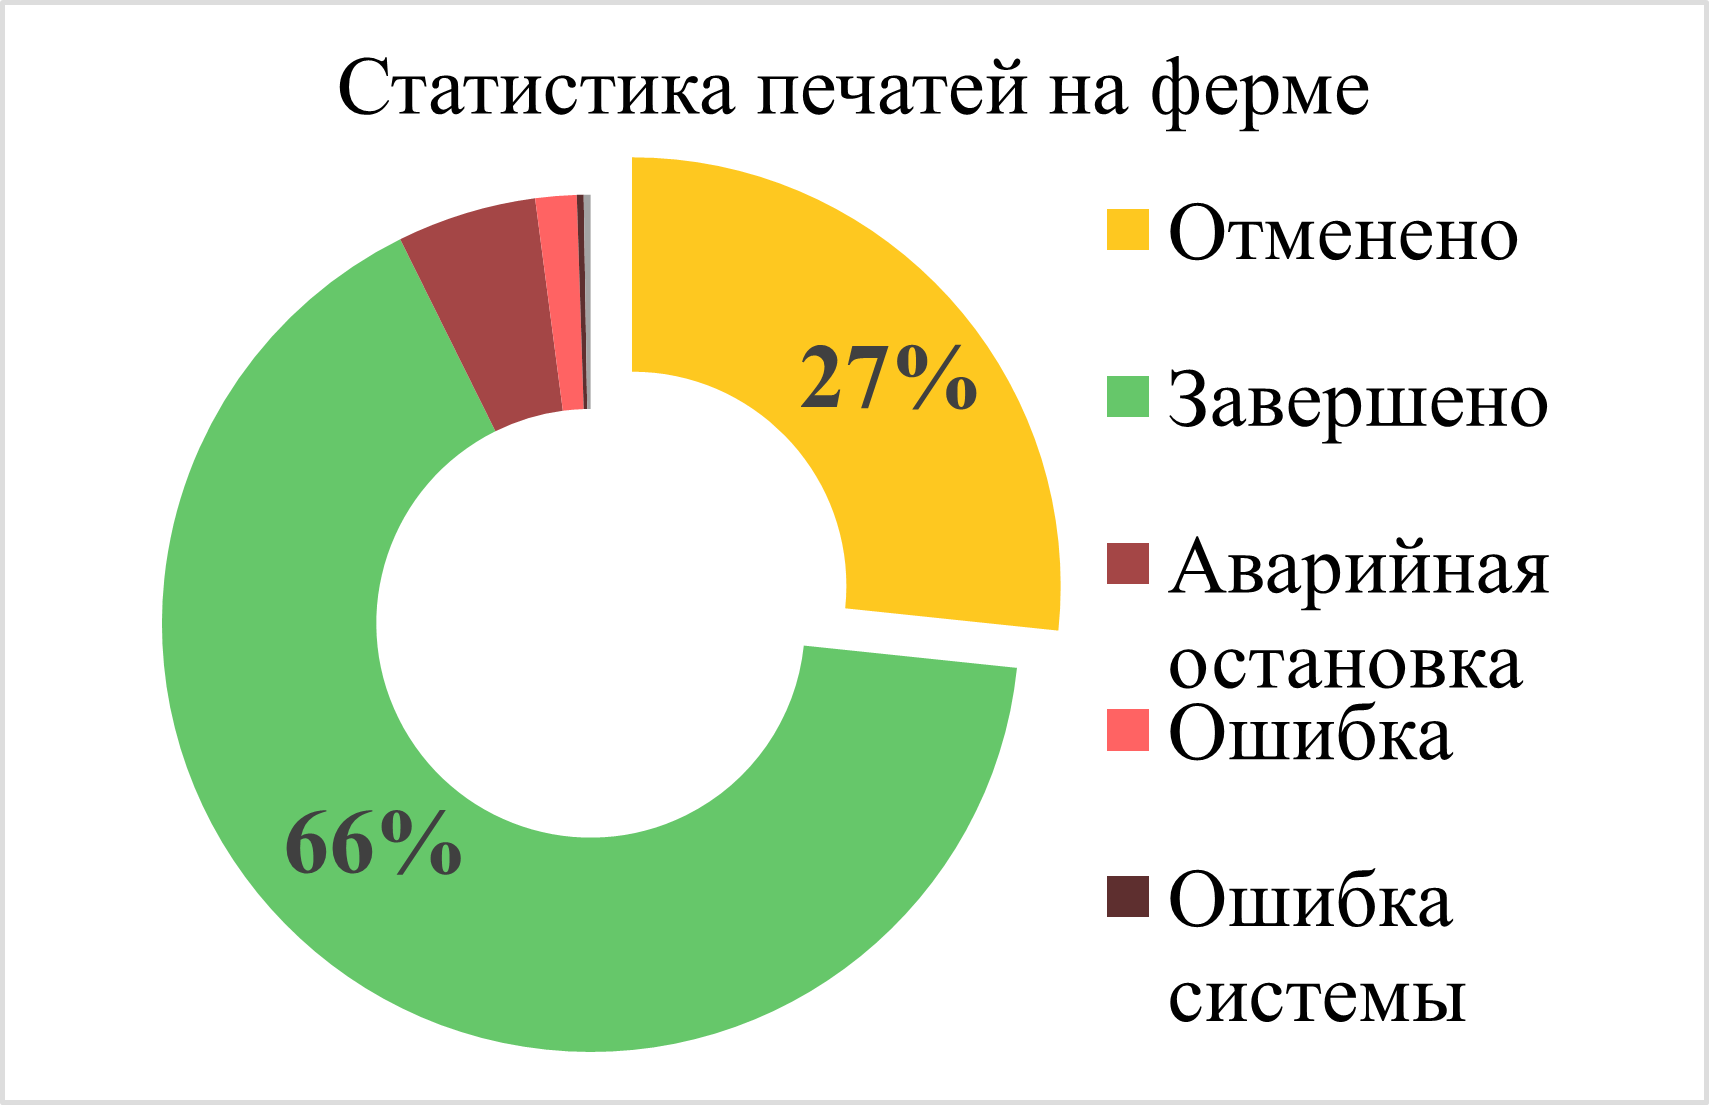
\includegraphics[width=0.9\hsize,trim=0.5mm 0.5mm 0.5mm 0.5mm,clip]{fig/printer-job-statuses.png}
  \caption{Распределение заданий по статусам на ферме 3D-принтеров компании Stereotech}
  \label{fig:stereotech-print-statuses}
\end{figure}

Статус задания описывает результат его выполнения в журнале принтера, но не подтверждает качество изделия и не определяет причину прекращения печати. Часть отмен связана с дефектом или с решением оператора по иной причине. Завершенное задание также может содержать дефект. Поэтому долю отмен нельзя использовать как частоту возникновения дефектов или общий процент брака. Полученные данные характеризуют эксплуатацию фермы до оценки предлагаемого контура контроля. Снижение числа отмен или расхода материала после его внедрения по этой сводке не измерялось.

\section{Методы мониторинга процесса печати и подходы к раннему обнаружению отклонений}

Ручной визуальный контроль дает оператору возможность оценивать состояние печати без сложной инфраструктуры. Его ограничения связаны с необходимостью постоянного присутствия человека и субъективностью оценки. При длительных заданиях или одновременной работе нескольких принтеров такой контроль не обеспечивает одинаковую скорость реакции.

Алгоритмический анализ изображений с применением машинного обучения используется для обнаружения и локализации аномалий в зоне печати. Он снижает зависимость наблюдения от оператора, но качество распознавания определяется полнотой и репрезентативностью обучающих данных. Недостаточная настройка критериев может приводить к ложным срабатываниям и пропускам событий.

Для рассматриваемой задачи выбран автоматизированный визуальный мониторинг с обнаружением «спагетти» во время печати и передачей признака нарушения в контур управления. Интервал получения кадров и время их анализа определяют задержку обнаружения отклонения.

Остановка задания должна опираться на подтверждение дефекта по нескольким наблюдениям, чтобы единичное срабатывание не прерывало исправную печать. Неопределенный результат при отсутствии достоверной оценки не должен вызывать управляющее действие.

